\begin{name}
	{\tenchude}
	{\tendethi}
	{\tentruong}
	{\thoigian}
\end{name}
%\part{ĐỀ ÔN TẬP}
% \subsection{Đề 7}
\Opensolutionfile{ans}[ans/ans-OTTNTHPT-DE7-LC]
\caulc
%Câu 1
\begin{ex}%[2D1V1-3]
	Có bao nhiêu số nguyên $m$ để hàm số $y=-x^3-3(m+1)x^2+3(m+1)x-1$ nghịch biến trên $\mathbb{R}$?
	\choice
	{$3$}
	{\True $2$}
	{$1$}
	{$0$}
	\loigiai{
		Ta có $y'=-3x^2-6(m+1)x+3(m+1)$.\\ 
		Hàm số nghịch biến trên $\mathbb{R}\Leftrightarrow y'\leq 0$ với mọi $x\in \mathbb{R}$.\\ 
		$\Leftrightarrow \Delta '=3\left[3(m+1)\right]^2-(-3)\cdot(3m+1)=9(m+1)^2+9(m+1)=9(m+1)(m+2)\leq 0$.\\ 
		$\Leftrightarrow-2\leq m\leq -1$.\\ 
		Vậy có hai giá trị $m$ nguyên thoả mãn yêu cầu là $m=-2$, $m=-1$.
	}
\end{ex}
%Câu 2
\begin{ex}%[2D1C2-1]
	Cho hàm số $y=\dfrac{x^2+2x+8}{x-2}$. Khẳng định nào sau đây \textbf{sai}?
	\choice
	{Hàm số đạt cực đại tại $x=-2$}
	{Hàm số đạt cực tiểu tại $x=6$}
	{\True Giá trị cực tiểu của hàm số là $y=6$}
	{Giá trị cực đại của hàm số là $y=-2$}
	\loigiai{
		Ta có $y'=\dfrac{x^2-4x-12}{(x-2)^2}$; $y'=0\Leftrightarrow x=-2$ hoặc $x=6$.\\ 
		Bảng biến thiên:
		\begin{center}
			
\begin{tikzpicture}[scale=1, font=\footnotesize, line join=round, line cap=round, >=stealth]
				\tkzTabInit[nocadre=false,lgt=1.2,espcl=2.5,deltacl=0.6] {$x$ /0.6,$y'$ /0.6,$y$ /2} {$-\infty$,$-2$,$2$,$6$,$+\infty$}
				\tkzTabLine{,+,0,-,d,-,0,+,}
				\tkzTabVar{-/$-\infty$,+/$-2$,-D+/$-\infty$/$+\infty$,-/$14$,+/$+\infty$}
			\end{tikzpicture}
		\end{center}
		Từ đó ta thấy giá trị cực tiểu của hàm số là $y=14$.
	}
\end{ex}
%Câu 3
\begin{ex}%[2D3H2-2]
	Cho hai mẫu số liệu ghép nhóm $A$ và $B$ có bảng tần số ghép nhóm như sau:
	\begin{center}
		$A$:
		\begin{tabular}{{|>{\centering\arraybackslash}m{3cm}|>{\centering\arraybackslash}m{2cm}|>{\centering\arraybackslash}m{2cm}|>{\centering\arraybackslash}m{2cm}|>{\centering\arraybackslash}m{2cm}|>{\centering\arraybackslash}m{2cm}|}}
			\hline
			Nhóm&$[1{,}6;1{,}8)$&$[1{,}8;2{,}0)$&$[2{,}0;2{,}2)$&$[2{,}2;2{,}4)$&$[2{,}4;2{,}6)$\\ 
			\hline
			Tần số&$12$&$25$&$18$&$10$&$2$\\ 
			\hline
		\end{tabular}
	\end{center}
	\begin{center}
		$B$:
		\begin{tabular}{{|>{\centering\arraybackslash}m{3cm}|>{\centering\arraybackslash}m{2cm}|>{\centering\arraybackslash}m{2cm}|>{\centering\arraybackslash}m{2cm}|>{\centering\arraybackslash}m{2cm}|>{\centering\arraybackslash}m{2cm}|}}
			\hline
			Nhóm&$[5{,}0;5{,}2)$&$[5{,}2;5{,}4)$&$[5{,}4;5{,}6)$&$[5{,}6;5{,}8)$&$[5{,}8;6{,}0)$\\ 
			\hline
			Tần số&$2$&$10$&$18$&$25$&$12$\\ 
			\hline
		\end{tabular}
	\end{center}
	Gọi $S_A$ và $S_B$ lần lượt là độ lệch chuẩn của mẫu số liệu ghép nhóm $A$ và $B$. Khẳng định nào sau đây đúng?
	\choice
	{\True $S_A=S_B$}
	{$3S_A=S_B$}
	{$S_B=S_A+3{,}4$}
	{$\left|S_A=S_B\right|>3{,}4$}
	\loigiai{
		Áp dụng công thức tính độ lệch chuẩn của mẫu số liệu ghép nhóm, ta có $S_A=S_B$.
	}
\end{ex}
%Câu 4
\begin{ex}%[1D6V4-2]
	Nghiệm của phương trình $3^{3x-2}=9^x$ là
	\choice
	{$x=4$}
	{$x=1$}
	{\True $x=2$}
	{$x=3$}
	\loigiai{
		$3^{3x-2}=9^x\Leftrightarrow 3^{3x-2}=3^{2x}\Leftrightarrow 3x-2=2x\Leftrightarrow x=2$.
	}
\end{ex}
%Câu 5
\begin{ex}%[0H5V3-6]
	Cho hai véc-tơ $\overrightarrow{a}$, $\overrightarrow{b}$ thoả mãn điều kiện là $|\overrightarrow{a}|=1$, $\left|\overrightarrow{b}\right|=2$ và $\overrightarrow{a}\cdot \overrightarrow{b}=-1$. Khi đó $\left|\overrightarrow{a}-\overrightarrow{b}\right|$ bằng
	\choice
	{\True $\sqrt{7}$}
	{$\sqrt{5}$}
	{$3$}
	{$1$}
	\loigiai{
		$\left(\overrightarrow{a}-\overrightarrow{b}\right)^2=\overrightarrow{a}^2-2\cdot \overrightarrow{a}\cdot \overrightarrow{b}+\overrightarrow{b}^2=\left|\overrightarrow{a}\right|^2-2\overrightarrow{a}\cdot \overrightarrow{b}+\left|\overrightarrow{b}\right|^2=7$. Suy ra $\left|\overrightarrow{a}-\overrightarrow{b}\right|=\sqrt{\left(\overrightarrow{a}-\overrightarrow{b}\right)^2}=\sqrt{7}$.
	}
\end{ex}
%Câu 6
\begin{ex}%[1D2V3-4]
	Cho cấp số nhân $\left(u_n\right)$, biết $u_2\cdot u_6=64$. Giá trị của $u_3\cdot u_5$ là
	\choice
	{$-8$}
	{$-64$}
	{\True $64$}
	{$8$}
	\loigiai{
		Ta có $u_3\cdot u_5=u_2\cdot q\cdot u_5=u_2\cdot u_6=64$.
	}
\end{ex}
%Câu 7
\begin{ex}%[2D1V3-1]
	\immini[thm]{Giá trị lớn nhất của hàm số có đồ thị ở Hình 1 trên đoạn $[-3;3]$ là
		\choice
		{$2$}
		{$-2$}
		{$3$}
		{\True $4$}
		\loigiai{
			Quan sát đồ thị, ta thấy giá trị lớn nhất của hàm số là $y=4$ khi $x=3$ hoặc $x=-3$.
	}}{\begin{tikzpicture}[scale=0.5, font=\footnotesize, line join=round, line cap=round, >=stealth]
			\draw[->] (-4,0)--(4,0) node[above] {$x$};
			\draw[->] (0,-3)--(0,5) node[left] {$y$};
			\foreach \x/\y in {-3/-2,-2/-1,-1/1,1/2,2/3,3/4} {
				\draw (\x,-0.1)--(\x,0.1) (-0.1,\y)--(0.1,\y);
			}
			\draw[dashed] (-3,0)--(-3,4)--(3,4)--(3,0) (-2,0)--(-2,-2)--(2,-2)--(2,0);
			\foreach \x/\g in {-3/-90,-2/135,-1/135,1/-135,2/90,3/-90}{
				\node at ($(\x,0)+(\g:6mm)$) {$\x$};
			}
			\foreach \x/\g in {-2/-135,-1/180,1/180,2/135,3/180,4/135}{
				\node at ($(0,\x)+(\g:6mm)$) {$\x$};
			}
			\node at ($(0,0)+(-135:6mm)$) {$O$};
			\draw[samples=100] plot[domain=-3:3](\x,{(\x)^4/4-2*(\x)^2+2});
		\end{tikzpicture}\\ 
		\centering{\textit{Hình 1}}}
\end{ex}
%Câu 8
\begin{ex}%[1D6V4-3]
	Tập nghiệm của bất phương trình $\log _2(x+2)\geq \log _2(6-x)$ là
	\choice
	{$(-2;3]$}
	{\True $[2;6)$}
	{$[2;+\infty )$}
	{$(-\infty; 2]$}
	\loigiai{
		$\log _2(x+2)\geq \log _2(6-x)\Leftrightarrow \heva{&x+2\geq 6-x\\&6-x>0}
		\Leftrightarrow \heva{&x\geq 2\\&x<6}\Leftrightarrow x\in [2;6)$.
	}
\end{ex}
%Câu 9:
\begin{ex}%[2H2N2-2]
	Trong không gian $Oxyz$, cho điểm $A(-3;2;-1)$. Toạ độ điểm $A'$ là hình chiếu vuông góc của điểm $A$ trên trục $Oz$ là
	\choice
	{\True $(0;0;-1)$}
	{$(-3;2;0)$}
	{$(-3;0;0)$}
	{$(0;2;0)$}
	\loigiai{
		$A'$ là hình chiếu vuông góc của $A$ trên $Oz$ suy ra $x_{A'}=0$, $y_{A'}=0$, $z_{A'}=z_A=-1$.\\ 
		Vậy $A'(0;0;-1)$.
	}
\end{ex}
%Câu 10
\begin{ex}%[2D4V2-4]
	Giá trị của $\displaystyle \int \limits _2^2\left( 2x-e^x\right)\mathrm{\,d}x$ bằng
	\choice
	{$3-e^2$}
	{$3-e$}
	{\True $5-e^2$}
	{$5-e$}
	\loigiai{
		$\displaystyle \int \limits _2^2\left( 2x-e^x\right)\mathrm{\,d}x=\left.\left(x^2-e^x\right)\right|_0^2=\left(4-e^2\right)-\left(0-e^0\right)=5-e^2$.
	}
\end{ex}
%Câu 11
\begin{ex}%[1H8C6-1]
	\immini[thm]{Cho hình chóp $S.ABC$ có $SA\perp (ABC)$, $SA=4a\sqrt{3}$, tam giác $ABC$ vuông tại $B$, $AB=2a$ và $BC=2\sqrt{3}a$ (Hình 2).
		Góc giữa đường thẳng $SC$ và mặt phẳng $(ABC)$ bằng
		\choice
		{$30^{\circ}$}
		{$45^{\circ}$}
		{$90^{\circ}$}
		{\True $60^{\circ}$}}{\begin{tikzpicture}[scale=0.5, font=\footnotesize, line join=round, line cap=round, >=stealth]
			\coordinate (A) at (0,0);
			\coordinate (B) at (2,-2);
			\coordinate (C) at (3,0);
			\coordinate (S) at (0,4);
			\draw (S)--(A)--(B)--(C)--(S)--(B);
			\draw[dashed] (A)--(C);
			\foreach \x/\y in {A/180,B/-90,C/0,S/90}{\draw[fill=black] (\x) circle (1pt) ($(\x)+(\y:6mm)$) node {$\x$};}
			\foreach \x/\y/\z in {S/A/C,S/A/B,A/B/C}{\tkzMarkRightAngles(\x,\y,\z);}
		\end{tikzpicture}\\ 
		\centering{\textit{Hình 2}}}
	\loigiai{
		Ta có $\heva{&SA\perp (ABC)\\&SC\cap (ABC)=C}$ nên $AC$ là hình chiếu vuông góc của $SC$ lên $ABC$.\\ 
		Suy ra $\left(SC,(ABC)\right)=\left(SC,AC\right)=\widehat{SCA}$ (do tam giác $SAC$ vuông tại $A$).\\ 
		Xét $\triangle ABC$ có $AC=\sqrt{AB^2+BC^2}=\sqrt{4a^2+12a^2}=4a$.\\ 
		Xét $\triangle SAC$ có $\tan \widehat{SCA}=\dfrac{SA}{AC}=\dfrac{4a\sqrt{3}}{4a}=\sqrt{3}$.\\ 
		Vậy góc giữa $SC$ và mặt phẳng $ABC$ bằng $60^{\circ}$
	}
\end{ex}
%Câu 12
\begin{ex}%[2H5V3-3]
	Trong không gian $Oxyz$, cho hai điểm $I(1;-2;1)$ và $A(1;2;3)$. Phương trình mặt cầu có tâm $I$ và đi qua $A$ là
	\choice
	{\True $(x-1)^2+(y+2)^2+(z-1)^2=20$}
	{$(x+1)^2+(y-2)^2+(z+1)^2=5$}
	{$(x+1)^2+(y-2)^2+(z+1)^2=20$}
	{$(x-1)^2+(y+2)^2+(z-1)^2=5$}
	\loigiai{
		Ta có $R=IA=\sqrt{(1-1)^2+\left[2-(2)\right]^2+(3-1)^2}=2\sqrt{5}$.\\ 
		Phương trình mặt cầu có tâm $I$ và đi qua $A$ là $(x-1)^2+(y+2)^2+(z-1)^2=20$. 
	}
\end{ex}
\Closesolutionfile{ans}
% \indapan{6}{ans/ans-OTTNTHPT-DE7-LC}
\cauds
\Opensolutionfile{ans}[ans/ans-OTTNTHPT-DE7-DS]
\begin{ex}%[2D1H5-3]
	Cho hàm số $y=f(x)$ liên tục trên $\mathbb{R}$ và có bảng biến thiên như sau
	\begin{center}
		
\begin{tikzpicture}
			\tkzTabInit[nocadre=false,lgt=1.2,espcl=2.5,deltacl=0.6]
			{$x$ /0.6, $y'$ /0.6, $y$ /2.5}
			{$-\infty$,$-5$,$-2$,$+\infty$}
			\tkzTabLine{,-,$0$,+,$0$,-,}
			\tkzTabVar{+/$6$,-/$-2$,+/$3$,-/$1$}
		\end{tikzpicture}
	\end{center}
	\choiceTF
	{\True Hàm số có hai cực trị}
	{Hàm số có hai tiệm cận ngang là $y=-2$ và $y=3$}
	{Hàm số có giá trị lớn nhất là $6$ và giá trị nhỏ nhất là $-2$}
	{Phương trình $f(x)=m-1$ có nghiệm khi $-1 \leq m \leq 7$}	
	\loigiai{
		Quan sát bảng biến thiên ta thấy
		\begin{itemchoice}
			\itemch Hàm số có hai cực trị là $x=-2$, $x=3$.
			\itemch Hàm số có hai tiệm cận ngang là $y=6$ và $y=1$.	
			\itemch Hàm số không có giá trị lớn nhất.
			\itemch Phương trình $f(x)=m-1$ có nghiệm khi $-2\leq m-1<6$ hay $-1 \leq m < 7$.
		\end{itemchoice}
	}
\end{ex}
\begin{ex}%[2D4V3-1]
	\immini{
		Cho hàm số $y=x^3-2 x^2-3 x+4$ có đồ thị $(C)$ và đường thẳng $d\colon y=2 x-2$.
		\choiceTF
		{\True Đồ thị $(C)$ và đường thẳng $d$ cùng đi qua các điểm $M(-2;-6)$, $N(1; 0)$, $P(3;4)$}
		{Diện tích hình phẳng giới hạn bởi đồ thị $(C)$, đường thẳng $d$ và hai đường thẳng $x=-2$, $x=1$ là $S_1=16$}
		{\True Diện tích hình phẳng giới hạn bởi đồ thị $(C)$ và đường thẳng $d$ là $S=\frac{253}{12}$}
		{Nếu diện tích hình phẳng giới hạn bởi đồ thị $(C)$, đường thẳng $d$ và hai đường thẳng $x=1$, $x=3$ là $S_2$ thì $S_1=3 S_2$}
	}
	{\begin{tikzpicture}[scale=.6,font=\footnotesize,samples=200,>=stealth]
			\tikzset{declare function={
					a=1;b=-2;c=-3;d=4; 
					xmin=-3;xmax=6;ymin=-7;ymax=6;}}
			%					\draw[color=gray!50,dashed] (xmin,ymin) grid (xmax,ymax);
			\draw[->] (xmin,0)--(xmax,0) node[below]{$x$};
			\draw[->] (0,ymin)--(0,ymax) node[left]{$y$};			
			\clip (xmin+0.1,ymin+0.1) rectangle (xmax-0.1,ymax-0.1);			
			\draw[dashed] (-2,0)|-(0,-6) (3,0)|-(0,4);
			\draw[teal,very thick] plot[domain=xmin+0.1:xmax-0.75](\x,{a*(\x)^3+b*(\x)^2+c*(\x)+d});
			\draw[violet,very thick] plot[domain=-2.2:4](\x,{2*(\x)-2});
			\foreach \x in {1,2,...,4}{
				\draw[thin] (\x,1.5pt)--(\x,-1.5pt);
				\draw[thin] (-\x,1.5pt)--(-\x,-1.5pt);}
			\foreach \y in {1,2,...,6}{
				\draw[thin] (1.5pt,\y)--(-1.5pt,\y);
				\draw[thin] (1.5pt,-\y)--(-1.5pt,-\y);}
			\draw[fill=white] 
			(-2,0) circle (0.05) node[above]{$-2$} 
			(1,0) circle (0.05) node[below]{$1$}
			(3,0) circle (0.05) node[below]{$3$}
			(0,4) circle (0.05) node[left]{$4$}			
			(0,-2) circle (0.05) node[left]{$-2$}
			(0,-6) circle (0.05) node[right]{$-6$}
			(0,5) circle (0.05) node[left]{$5$}
			; 		
			\draw[fill=red] (0,0) circle (0.07)node [below left]{$O$};
			\fill[pattern=vertical lines,opacity=0.3] plot[domain=1:3](\x,{2*(\x)-2})--plot[domain=3:1](\x,{a*(\x)^3+b*(\x)^2+c*(\x)+d});
			\draw[fill=red] (0,0) circle (0.07)node [below left]{$O$};
			\fill[pattern=grid,opacity=0.3] plot[domain=-2:1](\x,{2*(\x)-2})--plot[domain=1:-2](\x,{a*(\x)^3+b*(\x)^2+c*(\x)+d});			
			\draw 
			(4.5,4.0) node {$y=2x-2$}
			(0,-2.5) node[right] {$y=x^3-2x^2-3x+4$}
			(-0.5,1) node {$S_1$}
			(2,0.5) node {$S_2$}
			;
		\end{tikzpicture}
	}
	\loigiai{
		\begin{itemchoice}
			\itemch Đồ thị $(C)$ và đường thẳng $d$ cùng đi qua các điểm $M(-2;-6)$, $N(1;0)$, $P(3;4)$.
			\itemch $S_1=\displaystyle\int\limits_{-2}^1 (x^3-2x^2-3x+4-2x+2) \mathrm{\,d}x=\displaystyle\int\limits_{-2}^1 (x^3-2x^2-5x+6) \mathrm{\,d}x=\dfrac{63}{4}$.		
			\itemch 
			$S_1=\displaystyle\int\limits_{-2}^3 \left| x^3-2x^2-3x+4-2x+2\right|  \mathrm{\,d}x=\displaystyle\int\limits_{-2}^3 \left| x^3-2x^2-5x+6\right|  \mathrm{\,d}x=\dfrac{253}{12}$.
			\itemch 
			$S_2=S-S_1=\dfrac{253}{12}-\dfrac{63}{4}=\dfrac{16}{3}\Rightarrow\dfrac{S_1}{S_2}=\dfrac{189}{64}$.
		\end{itemchoice}
	}
\end{ex}
\begin{ex}%[2D6V1-4]
	Bạn An chơi tung đồng xu đổi bóng bay. Mỗi lượt chơi, An sẽ tung một đồng xu cân đối và đồng chất. Nếu đồng xu xuất hiện mặt ngửa, An được thưởng thêm $1$ quả bóng bay, ngược lại, An sẽ mất $1$ quả bóng bay bạn đang có. An đang có $10$ quả bóng bay.
	\choiceTF
	{\True Xác suất để An có $11$ quả bóng bay sau một lượt chơi là $\dfrac{1}{2}$}
	{\True Xác suất để An có $10$ quả bóng bay sau hai lượt chơi biết rằng An thắng ở lượt chơi thứ nhất là $\dfrac{1}{2}$}
	{Xác suất để An có $12$ quả bóng bay sau $3$ lượt chơi là $\dfrac{3}{8}$}
	{\True Sau $4$ lượt chơi, xác suất để An có $8$ quả bóng bay bằng xác suất để An có $12$ quả bóng bay}
	\loigiai{
		\begin{itemchoice}
			\itemch Vì An đang có $10$ quả bóng bay nên xác suất để An có $11$ quả bóng bay sau một lượt chơi bằng xác suất của biến cố \lq\lq An tung được mặt ngửa ở lượt chơi đầu tiên \rq\rq. Xác suất của biến cố này bằng $\dfrac{1}{2}$.
			\itemch Nếu An thắng ở lượt đầu tiên thì bạn sẽ có $11$ quả bóng bay.\\ Xác suất để An có $10$ quả bóng bay sau hai lượt chơi biết rằng bạn thắng ở lượt chơi thứ nhất bằng xác suất của biến cố \lq\lq An tung được mặt sấp ở lượt chơi thứ hai\rq\rq.\\ Xác suất của biến cố này bằng $\dfrac{1}{2}$.
			\itemch Sau mỗi lượt chơi An được hoặc mất $1$ quả bóng bay.\\ Do đó, sau một số lẻ lần chơi, số bóng của An sẽ là số lẻ.\\ Vậy xác suất để An có $12$ quả bóng bay sau $3$ lượt chơi là $0$.
			\itemch Xác suất để An có $8$ quả bóng bay sau $4$ lượt chơi bằng xác suất An tung được $3$ lần sấp và $1$ lần ngửa.\\
			Xác suất để An có $12$ quả bóng bay sau $4$ lượt chơi bằng xác suất An tung được $3$ lần ngửa và $1$ lần sấp.\\
			Do xác suất tung được mặt sấp bằng xác suất tung được mặt ngửa ở mỗi lần tung nên sau $4$ lượt chơi, xác suất để An có $8$ quả bóng bay bằng xác suất để An có $12$ quả bóng bay.
				\end{itemchoice}
		}
\end{ex}
\begin{ex}%[2H5V2-8]
	\immini[thm]{Các thiên thạch có đường kính lớn hơn $140$ m và có thể lại gần Trái Đất ở khoảng cách nhỏ hơn $7\,500\,000$ km được coi là những vật thể có khả năng va chạm gây nguy hiểm cho Trái Đất. Để theo dõi những thiên thạch này, người ta đã thiết lập các trạm quan sát các vật thể bay gần Trái Đất. Giả sử có một hệ thống quan sát có khả năng theo dõi các vật thể ở độ cao không vượt quá $6\,630$ km so với mực nước biển. Coi Trái Đất là khối cầu có bán kính $6\,370$ km.
	}
	{\begin{tikzpicture}[scale=.8,declare function={r=4;}]
			\path (0,0) coordinate (O)
			(0:r) coordinate (A)
			(0:r-1.5) coordinate (B)
			;
			
			\draw (O)--(B) node[above,pos=0.5,sloped]{\small$6370$ km};
			\draw (A)--(B) node[below,pos=0.5,sloped]{\tiny$6630$ km};
			
			\draw let \p1=($(O) - (A)$) in (O) circle ({veclen (\x1,\y1)});
			\draw let \p1=($(O) - (B)$) in (O) circle ({veclen (\x1,\y1)});
			\draw[<->] (O)--(B);
			\draw[<->] (A)--(B);
			\path let \p1=($ (O) - (A) $) in ($(O)+(35:{veclen(\x1,\y1)})$) coordinate (B);
			\path let \p1=($ (O) - (A) $) in ($(O)+(105:{veclen(\x1,\y1)})$) coordinate (A);
			\path ($(A)!-1/3!(B)$) coordinate (M);
			\path ($(A)!4/3!(B)$) coordinate (N);
			\draw (M)--(N);
			\foreach \t/\g in {M/90,A/90,O/-90,B/90}{
				\draw[fill=white] (\t) circle (1pt) node[shift={(\g:7pt)},font=\scriptsize]{$ \t $};
			}
	\end{tikzpicture}}
	\noindent
	Chọn hệ trục toạ độ $Oxyz$ trong không gian có gốc $O$ tại tâm Trái Đất và đơn vị độ dài trên mỗi trục toạ độ là $1\,000$ km. Một thiên thạch (coi như một hạt) chuyển động với tốc độ không đổi theo một đường thẳng từ điểm $M(6;15;-2)$, sau một thời gian vị trí đầu tiên thiên thạch di chuyển vào phạm vi theo dõi của hệ thống quan sát là điểm $A(5;12;0)$.
	\choiceTF
	{\True Đường thẳng $AM$ có phương trình chính tắc là $\dfrac{x-5}{1}=\dfrac{y-12}{3}=\dfrac{z}{-2}$}
	{Trên hệ trục toạ độ đã cho, thiên thạch di chuyển qua điểm $N(7; 18;-5)$}
	{\True Vị trí cuối cưng mà thiên thạch di chuyên trong phạm vi theo dõi cua hệ thống quan sát là $B\left(-\dfrac{6}{7};-\dfrac{39}{7};\dfrac{82}{7}\right)$}
	{\True Khoảng cách giữa vị trí đầu tiên và vị trí cuối cùng mà thiên thạch di chuyển trong phạm vi theo dơi của hệ thóng quan sát (làm tròn đên hàng đơn vị cua kilômét) là $21\,915$ km}
			\loigiai{
			\begin{itemchoice}
				\itemch Dường thẳng $AM$ đi qua $A(5;12;0)$ và có vectơ chỉ phương là $\overrightarrow{AM}=(1;3;-2)$ nên có phương trình chính tắc là $\dfrac{x-5}{1}=\dfrac{y-12}{3}=\dfrac{z}{-2}$.
				\itemch Thay toạ độ điểm $N(7;18;-5)$ vào phương trình $AM$ ta được
				\[\dfrac{7-5}{1}=\dfrac{18-12}{3}\neq \dfrac{-5}{-2}.\]
				 Suy ra thiên thạch không di chuyển qua điểm $N(7;18;-5)$.
				\itemch Vị trí cuối cùng mà thiên thạch di chuyển trong phạm vi theo dõi của hệ thống quan sát
				là $B\in AM\colon \dfrac{x-5}{1}=\dfrac{y-12}{3}=\dfrac{z}{-2} \Rightarrow B(5+t; 12+3t;-2t)$.\\
				Ngoài thực tế, khoảng cách từ tâm Trái Đất đến vị trí cuối cùng mà thiên thạch di chuyển trong phạm vi theo dõi của hệ thống quan sát là $6370+6630=13\,000$ (km) ứng với $13$ đơn vị trên hệ trục toạ độ, hay
				\allowdisplaybreaks
				\begin{eqnarray*}
					OB=13&\Leftrightarrow&OB^2=169\\
					&\Leftrightarrow &(5+t)^2+(12+3t)^2+(-2t)^2=169\\
					&\Leftrightarrow & 14 t^2+82 t=0 \Leftrightarrow \hoac{&t=0\\
						&t=-\dfrac{41}{7}.}
				\end{eqnarray*}
				Với $t=0\Rightarrow B(5;12;0)\equiv A$ (loại).\\
				Với $t=-\dfrac{41}{7}\Rightarrow B\left(-\dfrac{6}{7};-\dfrac{39}{7}; \dfrac{82}{7}\right)$.
				\itemch Khoảng cách giữa vị trí đầu tiên và vị trí cuối cùng mà thiên thạch di chuyển trong phạm vi theo dõi của hệ thống quan sát là khoảng cách giữa $A$ và $B$.\\
				Ta có $AB=\sqrt{\left(-\dfrac{6}{7}-5\right)^2+\left(-\dfrac{39}{7}-12\right)^2+\left(\dfrac{82}{7}\right)^2}=\dfrac{41\sqrt{14}}{7}$.\\
				Khoảng cách thực tế là $1\,000\cdot AB=1\,000\cdot \dfrac{41\sqrt{14}}{7} \approx 21\,915$ (km).
				\end{itemchoice}
			}
\end{ex}
\Closesolutionfile{ans}
% \indapan{2}{ans/ans-OTTNTHPT-DE7-DS}
\Opensolutionfile{ans}[ans/ans-OTTNTHPT-DE7-KQ]
\caukq
%Câu 1
\begin{ex}%[2D1C3-6]
	\immini[thm]{Bạn Linh có một tấm bìa hình vuông cạnh dài $40$ cm. Bạn dự định cắt bỏ phần tô màu như Hình $5$a rồi gấp vào dán lại để làm một hộp quà dạng hình chóp tứ giác đều như Hình $5$b (các mép dán không đáng kể). Để hộp quà có thể tích lớn nhất thì diện tích của phần bìa bị cắt bỏ là bao nhiêu cen-ti-mét vuông?}{
		\begin{tikzpicture}[scale=1, font=\footnotesize, line join=round, line cap=round, >=stealth]
			\coordinate (A) at (0,0);
			\coordinate (B) at (2,0);
			\coordinate (C) at (2,2);
			\coordinate (D) at (0,2);
			\coordinate (E) at (0.5,0.5);
			\coordinate (F) at (1.5,0.5);
			\coordinate (G) at (1.5,1.5);
			\coordinate (H) at (0.5,1.5);
			\coordinate (I) at ($(A)!0.5!(B)$);
			\coordinate (J) at ($(B)!0.5!(C)$);
			\coordinate (K) at ($(C)!0.5!(D)$);
			\coordinate (L) at ($(D)!0.5!(A)$);
			\fill[cyan] (A)--(B)--(C)--(D)--cycle;
			\fill[white] (L)--(E)--(I)--(F)--(J)--(G)--(K)--(H)--cycle;
			\draw (A)--(B)--(C)--(D)--cycle (L)--(E)--(I)--(F)--(J)--(G)--(K)--(H)--cycle (I)--(J)--(K)--(L);
			\path (A)--(B) node[midway, below]{$a)$};
		\end{tikzpicture}
		\vspace{1cm}
		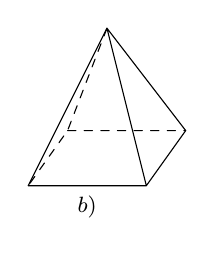
\begin{tikzpicture}[scale=1, font=\footnotesize, line join=round, line cap=round, >=stealth]
			\coordinate (A) at (0,0);
			\coordinate (B) at (-0.5,-0.7);
			\coordinate (C) at (1,-0.7);
			\coordinate (D) at (1.5,0);
			\coordinate (S) at (0.5,1.3);
			\draw[dashed] (S)--(A)--(B) (A)--(D);
			\draw (S)--(B)--(C)--(D)--(S)--(C);
			\path (B)--(C) node[midway, below] {$b)$};
		\end{tikzpicture}\\
		\centering{\textit{Hình 5}}
	}
	\par
	\shortans[]{960}
	\loigiai{
		Gọi $x$ (cm) là độ dài cạnh đáy của hộp quà dạng hình chóp tứ giác đều $(0<x<40)$.\\
		Chiều cao mặt bên của hình chóp là $\dfrac{40-x}{2}$ (cm).\\ 
		Chiều cao của hình chóp là $\sqrt{\left(\dfrac{40-x}{2}\right)^2-\left(\dfrac{x}{2}\right)^2}=\dfrac{1}{2}\sqrt{1\,600-80x}$ (cm).\\ 
		Thể tích của hộp quà là $V=\dfrac{1}{3}\cdot x^2\cdot \dfrac{1}{2}\sqrt{1\,600-80x}=\dfrac{1}{6}x^2\sqrt{1\,600-80x}$ (cm$^3$).\\ 
		Ta có $V'=\dfrac{5\sqrt{5}x(16-x)}{3\sqrt{20-x}}$, $V'=0\Leftrightarrow x=16$.\\ 
		Lập bảng biến thiên, ta thấy $V$ lớn nhất khi $x=16$.\\ 
		Khi đó diện tích của phần bìa cắt bỏ là $40\cdot 40-16\cdot 16-4\cdot \dfrac{1}{2}\cdot 16\cdot \dfrac{40-16}{2}=960$ (cm$^2$).
	}
\end{ex}
%Câu 2
\begin{ex}%[2D4V3-5]
	\immini[thm]{Một khối bê tông cao $2$ m được đặt trên mặt đất phẳng. Nếu cắt khối bê tông này bằng mặt phẳng nằm ngang, cách mặt đất $x$ (m) thì được mặt cắt là hình chữ nhật có chiều dài $5$ m, chiều rộng $(0{,}5)^x$ (m), trong đó $0\leq x\leq 2$ (Hình 6). Tính thể tích của khối bê tông (làm tròn kết quả đến hàng phần trăm của mét khối).}{
		\begin{tikzpicture}[scale=0.7, font=\footnotesize, line join=round, line cap=round, >=stealth]
			\begin{scope}[rotate around={-45:(2,4)}]
				\draw plot[domain=0.5:2,samples=100] (\x,{-(\x)^2});
				\draw plot[domain=3.5:5,samples=100] (\x,{-(\x-3)^2+2});
				\coordinate (B) at (0.5,{-(0.5)^2});
				\coordinate (C) at (2,{-(2)^2});
				\coordinate (D) at (3.5,{-(3.5-3)^2+2});
				\coordinate (E) at (5,{-(5-3)^2+2});
				\coordinate (K) at (1.5,{-(1.5)^2});
				\coordinate (L) at (4.5,{-(4.5-3)^2+2});
			\end{scope}
			\coordinate (F) at ($(B)+(0.5,0.3)$);
			\coordinate (G) at ($(D)+(0.5,0.3)$);
			\coordinate (H) at ($(F)-(0,3)$);
			\coordinate (I) at ($(G)-(0,3)$);
			\coordinate (J) at ($(F)!0.6!(H)$);
			\coordinate (M) at ($(G)!0.6!(I)$);
			\fill[pattern=north east lines] (J)--(K)--(L)--(M)--cycle;
			\draw (B)--(D) (C)--(E) (B)--(F) (G)--(D) (F)--(G)--(I)--(E) (K)--(L)--(M);
			\draw[dashed] (F)--(H)--(I) (H)--(C) (K)--(J)--(M) (G)--($(G)+(0.5,0.3)$) (M)--($(M)+(1,0.6)$) (I)--($(I)+(1,0.6)$);
			\path (J)--(M) node[midway, above, scale=1] {$5$ m}; 
			\draw[<->] ($(I)+(0.5,0.3)$)--($(G)+(0.5,0.3)$) node[midway, above right] {$2$ m};
			\draw[<->] ($(I)+(1,0.6)$)--($(M)+(1,0.6)$) node[midway, right] {$x$ (m)};
		\end{tikzpicture}\\ 
		\centering{\textit{Hình 6}}
	}
	\par
	\shortans[]{$5{,}41$}
	\loigiai{
		Chọn trục $Ox$ thẳng đứng, gốc $O$ nằm trên mặt đáy của khối bê tông, chiều dương hướng lên trên. Khi đó, khối bê tông nằm trong khoảng không gian giữa hai mặt phẳng vuông góc với $Ox$ lần lượt tại các điểm $x=0$ và $x=2$. Mặt phẳng vuông góc với $Ox$ tại điểm có hoành độ $x(0\leq x\leq 2)$ cắt khối bê tông theo mặt cắt có diện tích là $S(x)=5\cdot (0{,}5)^x$ (m$^2$).\\ 
		Do đó, thể tích của khối bê tông là
		\[V=\displaystyle \int \limits _0^2S(x)\mathrm{\,d}x=\displaystyle \int \limits _0^2 5\cdot (0{,}5)^x\mathrm{\,d}x=\left.\dfrac{5}{\ln 0{,}5}\cdot (0{,}5)^x\right|_0^2=-\dfrac{5}{\ln 0{,}5}\left(\dfrac{1}{4}-1\right)=\dfrac{15}{4\ln 2}\approx 5{,}41 \text{ m}^3.\]
	}
\end{ex}
%Câu 3
\begin{ex}%[2D6V1-4]
	Bạn Minh có 9 viên bi có cùng kích thước và khối lượng, $3$ cái hộp được sơn màu khác nhau. Mỗi cái hộp có thể chứa tối đa $9$ viên bi. Minh bỏ ngẫu nhiên $9$ viên bi vào $3$ cái hộp. Tính xác suất để mỗi hộp đều có $3$ viên bi, biết rằng hộp nào cũng có ít nhất $2$ viên bi.
	\par
	\shortans[]{$\dfrac{20}{137}$}
	\loigiai{
		Số cách bỏ bi vào hộp sao cho hộp nào cũng có $3$ viên bi là $C_9^3C_6^3=1\,680$.\\ 
		Số cách bỏ bi vào hộp sao cho có $1$ hộp có $2$ viên bi, $1$ hộp có $3$ viên bi và $1$ hộp có $4$ viên bi là $3\!C_9^2C_7^3=7\,560$.\\ 
		Số cách bỏ bi vào hộp sao cho có $2$ hộp có $2$ viên bi và $1$ hộp có $5$ viên bi là $3C_9^2C_7^3=2\,268$.\\ 
		Số cách bỏ bi vào hộp sao cho hộp nào cũng có ít nhất $2$ viên bi là
		\[1\,680+7\,560+2\,268=11\,508.\]
		Vậy xác suất để mỗi hộp đều có $3$ viên bi biết rằng hộp nào cũng có ít nhất $2$ viên bi là $\dfrac{1\,680}{11\,508}=\dfrac{20}{137}$.
	}
\end{ex}
%Câu 4
\begin{ex}%[1D2C3-7]
	Xét các số thực dương $x$, $y$, $z$ theo thứ tự đó lập thành một cấp số cộng, đồng thời, các số $x$, $y-3$, $z+10$ theo thứ tự đó lập thành một cấp số nhân. Biết rằng $x+y+z=24$. Giá trị của tích $xyz$ bằng bao nhiêu?
	\par
	\shortans[]{120}
	\loigiai{
		Từ giả thiết bài toán, ta có $\heva{&x+y+z=24\\&2y=x+z}\Rightarrow x=8$.\\ 
		Hơn nữa $\heva{&x+z=2y\\&(y-3)^2=x(z+10)}\Rightarrow \heva{&x+z=16\\ &25=x(z+10)}\Rightarrow \hoac{&x=1,\, z=15\\ &x=25,\, z=-9.}$\\ 
		Vậy ba số $x$, $y$, $z$ cần tìm theo yêu cầu của bài toán là $x=1$, $y=8$, $z=15$. Suy ra $xyz=120$.
	}
\end{ex}
%Câu 5
\begin{ex}%[2H2C2-6]
	\immini[thm]{Một căn phòng có dạng hình hộp chữ nhật $ABCD.EFGH$ với $AB=6$ m, $AD=8$ m và chiều cao $10$ m. Cần giăng một dây trang trí trong phòng từ điểm $G$ đến điểm $I$ thuộc mặt sàn của phòng, rồi từ điểm đó giăng tiếp đến vị trí điểm $M$ là trung điểm của $AF$ (Hình $7$). Biết rằng $I$ là điểm sao cho dây trang trí được dùng ít nhất, khi đó $I$ cahs góc phòng $B$ bao nhiêu mét (kết quả làm tròn đến hàng phần trăm)?}{
		\begin{tikzpicture}[scale=1, font=\footnotesize, line join=round, line cap=round, >=stealth]
			\coordinate (A) at (0,0);
			\coordinate (B) at (2,0);
			\coordinate (E) at (0,2);
			\coordinate (F) at (2,2);
			\coordinate (D) at (2.5,-1.5);
			\coordinate (C) at (4.5,-1.5);
			\coordinate (H) at (2.5,0.5);
			\coordinate (G) at (4.5,0.5);
			\coordinate (M) at ($(A)!0.5!(F)$);
			\fill[orange!40!white] (A)--(B)--(C)--(D)--cycle;
			\draw (C)--(D)--(A)--(E)--(F)--(G)--(H)--(E);
			\draw (G)--(C);
			\draw (H)--(D);
			\draw[dashed] (A)--(F);
			\foreach \x in {A,F,C} {\draw[dashed] (B)--(\x);};
			\foreach \x in {A,B,C,D,E,F,G,H,M} {\draw[fill=black] (\x) circle (1pt);};
			\node[left] at (A) {$A$};
			\node[left] at (M) {$M$};
			\node[below] at (D) {$D$};
			\node[below] at (C) {$C$};
			\node[right] at (B) {$B$};
			\foreach \x in {E,F,G,H} {\node[above] at (\x) {$\x$};};
		\end{tikzpicture}\\ 
		\centering{\textit{Hình 7}}
	}
	\par
	\shortans[]{$3{,}33$}
	\loigiai{
		\immini{Dựng hệ trục $Oxyz$ như hình vẽ.\\ 
			Khi đó toạ độ các điểm là $B(0;0;0)$, $C(8;0;0)$, $D(8;6;0)$, $A(0;6;0)$, $G(8;0;10)$, $F(0;0;10)$.\\ 
			Ta có $M$ là trung điểm của $AF$ nên $M(0;3;5)$\\ 
			Dây giăng từ điểm $G$ đến chạm mặt sàn tại điểm $I(x;y;0)\in (Oxy)$ với $0\leq x\leq 8$, $0\leq y\leq 6$.\\ 
			Gọi $N$ là điểm đối xứng của điểm $M$ qua $(Oxy)$ thì $N(0;3;-5).$}{
			\begin{tikzpicture}[scale=1, font=\footnotesize, line join=round, line cap=round, >=stealth]
				\coordinate (A) at (0,0);
				\coordinate (B) at (2,0);
				\coordinate (E) at (0,2);
				\coordinate (F) at (2,2);
				\coordinate (D) at (2.5,-1.5);
				\coordinate (C) at (4.5,-1.5);
				\coordinate (H) at (2.5,0.5);
				\coordinate (G) at (4.5,0.5);
				\coordinate (M) at ($(A)!0.5!(F)$);
				\coordinate (P) at ($(A)!0.5!(B)$);
				\coordinate (N) at ($(M)!2!(P)$);
				%\fill[orange!40!white] (A)--(B)--(C)--(D)--cycle;
				\draw (C)--(D)--(A)--(E)--(F)--(G)--(H)--(E);
				\draw (G)--(C);
				\draw (H)--(D);
				\draw[dashed] (A)--(F) (M)--(P)--(N)--(G);
				\foreach \x in {A,F,C} {\draw[dashed] (B)--(\x);};
				\foreach \x in {A,B,C,D,E,F,G,H,M,N} {\draw[fill=black] (\x) circle (1pt);};
				\node[left] at (A) {$A$};
				\node[left] at (M) {$M$};
				\node[below] at (D) {$D$};
				\node[below] at (C) {$C$};
				\node[below] at (N) {$N$};
				\node[right] at (B) {$B$};
				\foreach \x in {E,F,G,H} {\node[above] at (\x) {$\x$};};
				\draw[->] (F)--($(F)+(0,1)$) node[left] {$z$};
				\draw[->] (A)--($(A)+(-1,0)$) node[below] {$y$};
				\draw[->] (C)--($(C)+(0.5,-0.3)$) node[below] {$x$};
				\tkzMarkRightAngles(M,P,B);
				\coordinate (I) at ($(N)!0.3!(G)$);
				\draw[fill=black] (I) circle (1pt) node[below right] {$I$};
				\draw (N)--($(N)!0.2!(M)$) (N)--($(N)!0.1!(G)$);
			\end{tikzpicture}
		}
		Ta có $IM+IG=IN+IG\geq GN$.\\ 
		Để $IM+IG$ nhỏ nhất thì ba điểm $I$, $G$, $N$ thẳng hàng.\\ 
		Suy ra $\overrightarrow{IG}$, $\overrightarrow{NG}$ cùng phương.\\ 
		Ta có $\overrightarrow{IG}=(8-x;-y;10)$, $\overrightarrow{NG}=(8;-3;15)$.\\ 
		Do đó $\dfrac{8-x}{8}=\dfrac{-y}{-3}=\dfrac{10}{15}$. Suy ra $x\dfrac{8}{3}$, $y=2\Rightarrow I\left(\dfrac{8}{3};2;0\right)$.\\ 
		Vậy $IB=\sqrt{\left(\dfrac{8}{3}\right)^2+2^2}=\dfrac{10}{3}\approx 3{,}33$.
	}
\end{ex}
%Câu 6
\begin{ex}%[2CD2V1-1]
	Bác An muốn gửi tiết kiệm $200$ triệu đồng vào một ngân hàng trong một năm theo hình thức lãi kép (tức là hết mỗi kì hạn thì tiền lãi nhập vào gốc để tính lãi cho kì hạn tiếp theo). Bác An phân vân giữa hai lựa chọn
	\begin{itemize}
		\item Phương án 1: Gửi tiền với lãi suất $4{,}2\%$/năm, kì hạn $3$ tháng;
		\item Phương án 2: Gửi tiền với lãi suất $5{,}1\%$/năm, kì hạn $6$ tháng.
	\end{itemize}
	Biết rằng lãi suất ngân hàng không thay đổi trong năm đó, sau khi tính toán bác An lựa chọn phương án $2$. Tính số tiền có lợi hơn nếu bác An chọn phương án $2$ so với phương án $1$ (kết quả làm tròn đến hàng phần mười của triệu đồng).
	\par
	\shortans[]{$1{,}8$}
	\loigiai{
		Nếu gửi số tiền $A$, lãi suất $r\%$ cho mỗi kì hạn và sau $n$ kì hạn thì nhận được tổng số tiền là $T=A(1+r\%)^n$.\\ 
		Tổng số tiền bác An nhận được nếu gửi theo phương án $1$ là\\ 
		$T_1=200\left(1+\dfrac{3}{12}\cdot 4{,}2\%\right)^4$.\\ 
		Tổng số tiền bác An nhận được nếu gửi theo phương án $2$ là\\ 
		$T_2=200\left(1+\dfrac{6}{12}\cdot 5{,}1\%\right)^2$.\\ 
		Số tiền chênh lệch nếu bác An chọn phương án $2$ so với phương án $1$ là\\ 
		$T_2-T_1\approx 1{,}8$ (triệu đồng).
	}
\end{ex}
\Closesolutionfile{ans}
% \indapan{6}{ans/ans-OTTNTHPT-DE7-KQ}